\documentclass[14pt]{extbook}
\usepackage{multicol, enumerate, enumitem, hyperref, color, soul, setspace, parskip, fancyhdr} %General Packages
\usepackage{amssymb, amsthm, amsmath, bbm, latexsym, units, mathtools} %Math Packages
\everymath{\displaystyle} %All math in Display Style
% Packages with additional options
\usepackage[headsep=0.5cm,headheight=12pt, left=1 in,right= 1 in,top= 1 in,bottom= 1 in]{geometry}
\usepackage[usenames,dvipsnames]{xcolor}
\usepackage{dashrule}  % Package to use the command below to create lines between items
\newcommand{\litem}[1]{\item#1\hspace*{-1cm}\rule{\textwidth}{0.4pt}}
\pagestyle{fancy}
\lhead{Progress Quiz 10}
\chead{}
\rhead{Version A}
\lfoot{6232-9639}
\cfoot{}
\rfoot{Fall 2020}
\begin{document}

\begin{enumerate}
\litem{
First, find the equation of the line containing the two points below. Then, write the equation as $ y=mx+b $ and choose the intervals that contain $m$ and $b$.\[ (10, -3) \text{ and } (-10, -2) \]\begin{enumerate}[label=\Alph*.]
\item \( m \in [-0.3, -0.03] \hspace*{3mm} b \in [7.23, 8.07] \)
\item \( m \in [0, 0.19] \hspace*{3mm} b \in [-1.83, -1.23] \)
\item \( m \in [-0.3, -0.03] \hspace*{3mm} b \in [-14.06, -12.54] \)
\item \( m \in [-0.3, -0.03] \hspace*{3mm} b \in [1.51, 2.57] \)
\item \( m \in [-0.3, -0.03] \hspace*{3mm} b \in [-3.76, -2.48] \)

\end{enumerate} }
\litem{
Find the equation of the line described below. Write the linear equation as $ y=mx+b $ and choose the intervals that contain $m$ and $b$.\[ \text{Parallel to } 5 x + 8 y = 13 \text{ and passing through the point } (-8, 3). \]\begin{enumerate}[label=\Alph*.]
\item \( m \in [-1.21, -0.06] \hspace*{3mm} b \in [10.1, 11.1] \)
\item \( m \in [-1.21, -0.06] \hspace*{3mm} b \in [1.7, 3.5] \)
\item \( m \in [-1.21, -0.06] \hspace*{3mm} b \in [-3.6, -1.3] \)
\item \( m \in [-2.71, -1.36] \hspace*{3mm} b \in [-3.6, -1.3] \)
\item \( m \in [0.13, 0.91] \hspace*{3mm} b \in [7.9, 10.7] \)

\end{enumerate} }
\litem{
Find the equation of the line described below. Write the linear equation as $ y=mx+b $ and choose the intervals that contain $m$ and $b$.\[ \text{Perpendicular to } 8 x + 3 y = 13 \text{ and passing through the point } (5, 4). \]\begin{enumerate}[label=\Alph*.]
\item \( m \in [2.47, 3.05] \hspace*{3mm} b \in [0.6, 2.7] \)
\item \( m \in [0.32, 0.75] \hspace*{3mm} b \in [0.6, 2.7] \)
\item \( m \in [0.32, 0.75] \hspace*{3mm} b \in [-1.9, 0.4] \)
\item \( m \in [0.32, 0.75] \hspace*{3mm} b \in [-5.1, -1.5] \)
\item \( m \in [-0.54, -0.03] \hspace*{3mm} b \in [4.4, 7.6] \)

\end{enumerate} }
\litem{
First, find the equation of the line containing the two points below. Then, write the equation as $ y=mx+b $ and choose the intervals that contain $m$ and $b$.\[ (3, 9) \text{ and } (-10, 3) \]\begin{enumerate}[label=\Alph*.]
\item \( m \in [-0.1, 2.6] \hspace*{3mm} b \in [6.1, 8.4] \)
\item \( m \in [-0.1, 2.6] \hspace*{3mm} b \in [4.6, 7.4] \)
\item \( m \in [-0.1, 2.6] \hspace*{3mm} b \in [-10.8, -5.7] \)
\item \( m \in [-1.4, 0.3] \hspace*{3mm} b \in [-3.1, 2.3] \)
\item \( m \in [-0.1, 2.6] \hspace*{3mm} b \in [12.9, 15.1] \)

\end{enumerate} }
\litem{
Write the equation of the line in the graph below in Standard form $Ax+By=C$. Then, choose the intervals that contain $A, B, \text{ and } C$.
\begin{center}
    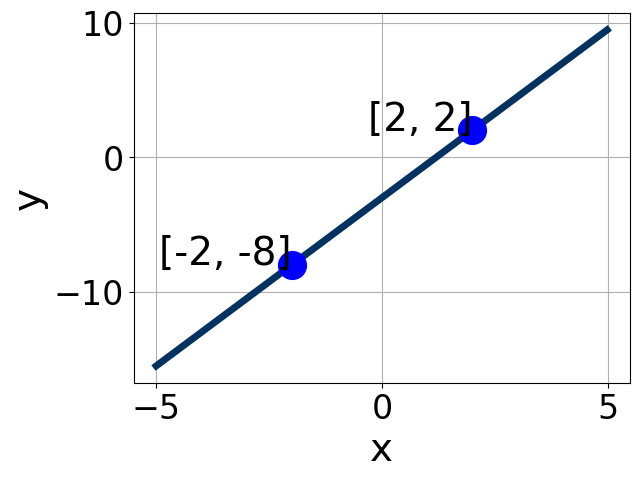
\includegraphics[width=0.5\textwidth]{../Figures/linearGraphToStandardCopyA.png}
\end{center}
\begin{enumerate}[label=\Alph*.]
\item \( A \in [3.1, 6.5], \hspace{3mm} B \in [1.93, 2.16], \text{ and } \hspace{3mm} C \in [-8.4, -5.6] \)
\item \( A \in [-5.7, -4.5], \hspace{3mm} B \in [1.93, 2.16], \text{ and } \hspace{3mm} C \in [-8.4, -5.6] \)
\item \( A \in [-4.3, -0.8], \hspace{3mm} B \in [0.43, 1.15], \text{ and } \hspace{3mm} C \in [-5.5, 0.3] \)
\item \( A \in [3.1, 6.5], \hspace{3mm} B \in [-2.82, -1.89], \text{ and } \hspace{3mm} C \in [3.8, 6.5] \)
\item \( A \in [-4.3, -0.8], \hspace{3mm} B \in [-1.14, -0.87], \text{ and } \hspace{3mm} C \in [-0.2, 3.2] \)

\end{enumerate} }
\litem{
Solve the equation below. Then, choose the interval that contains the solution.\[ -12(-15x -6) = -17(-3x + 2) \]\begin{enumerate}[label=\Alph*.]
\item \( x \in [-0.84, -0.6] \)
\item \( x \in [0.04, 0.49] \)
\item \( x \in [-0.6, -0.26] \)
\item \( x \in [-0.23, 0.01] \)
\item \( \text{There are no real solutions.} \)

\end{enumerate} }
\litem{
Solve the linear equation below. Then, choose the interval that contains the solution.\[ \frac{7x -9}{2} - \frac{8x -9}{7} = \frac{9x -5}{3} \]\begin{enumerate}[label=\Alph*.]
\item \( x \in [-1.15, 2.85] \)
\item \( x \in [-6.41, -5.41] \)
\item \( x \in [5.78, 9.78] \)
\item \( x \in [-2.41, -1.41] \)
\item \( \text{There are no real solutions.} \)

\end{enumerate} }
\litem{
Solve the linear equation below. Then, choose the interval that contains the solution.\[ \frac{-7x -3}{3} - \frac{-3x + 9}{7} = \frac{-7x -5}{6} \]\begin{enumerate}[label=\Alph*.]
\item \( x \in [0, 0.7] \)
\item \( x \in [-10.3, -8.7] \)
\item \( x \in [-2.6, -0.4] \)
\item \( x \in [1.3, 1.6] \)
\item \( \text{There are no real solutions.} \)

\end{enumerate} }
\litem{
Write the equation of the line in the graph below in Standard form $Ax+By=C$. Then, choose the intervals that contain $A, B, \text{ and } C$.
\begin{center}
    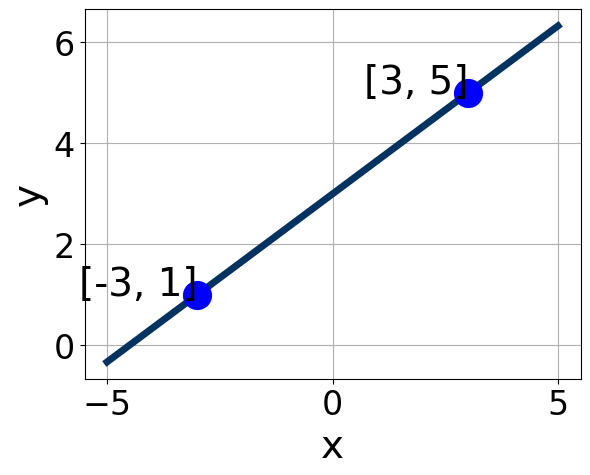
\includegraphics[width=0.5\textwidth]{../Figures/linearGraphToStandardA.png}
\end{center}
\begin{enumerate}[label=\Alph*.]
\item \( A \in [1.4, 3.3], \hspace{3mm} B \in [-3.26, -2.93], \text{ and } \hspace{3mm} C \in [-9, -8] \)
\item \( A \in [-1.7, -0.6], \hspace{3mm} B \in [0.56, 1.73], \text{ and } \hspace{3mm} C \in [3, 6] \)
\item \( A \in [-3.7, -1.7], \hspace{3mm} B \in [2.95, 4.21], \text{ and } \hspace{3mm} C \in [8, 16] \)
\item \( A \in [-1.7, -0.6], \hspace{3mm} B \in [-2.98, -0.93], \text{ and } \hspace{3mm} C \in [-5, 1] \)
\item \( A \in [1.4, 3.3], \hspace{3mm} B \in [2.95, 4.21], \text{ and } \hspace{3mm} C \in [8, 16] \)

\end{enumerate} }
\litem{
Solve the equation below. Then, choose the interval that contains the solution.\[ -10(4x + 14) = -11(9x -7) \]\begin{enumerate}[label=\Alph*.]
\item \( x \in [3.54, 4.14] \)
\item \( x \in [-0.9, 0.01] \)
\item \( x \in [-2.08, -0.99] \)
\item \( x \in [0.6, 1.74] \)
\item \( \text{There are no real solutions.} \)

\end{enumerate} }
\end{enumerate}

\end{document}